%%%%%%%%%%%%%%%%%%%%%%%%%%%%%%%%%%%%%%%%%%%%%%%%%%%%%%%%%%%%%%%%%%%%%%%%
% V2D Challenge 2026, Track 3 technical report (two-page extended abstract)
% Build:  pdflatex main && bibtex main && pdflatex main && pdflatex main
%%%%%%%%%%%%%%%%%%%%%%%%%%%%%%%%%%%%%%%%%%%%%%%%%%%%%%%%%%%%%%%%%%%%%%%%

\pdfoutput=1
\documentclass[10pt]{nvidiaextabstract}

\usepackage{microtype}
\usepackage{multirow}
\usepackage{subcaption}
\usepackage{xspace}

\venue{From Human Videos to Dexterous Robot Capability (CoRL 2026)}
\submissionID{Kiarash\_Ghasemzadeh8}

\title{Selecting, Not Smoothing: Physically Grounded Object Trajectories from Egocentric Video for Dexterous Robot Imitation}
\subtitle{V2D Challenge 2026 --- Track 3 Technical Report}
\shorttitle{Selecting, Not Smoothing: Egocentric Video to Robot Imitation}

\author[1]{Kiarash Ghasemzadeh}
\affil[1]{University of Alberta \& Amii}
\affil[ ]{\texttt{kghasemz@ualberta.ca}}

\begin{abstract}
\textbf{Abstract:}
We present our Track~3 system, which turns an egocentric stereo recording of a person manipulating kitchen objects into a
dexterous robot-hand policy in simulation. Using only our own reconstructions (no provided scans or motion capture), we
estimate metric object meshes, hand motion and 6-DoF object trajectories, ground them physically, and train one
policy per episode with soft actor-critic. Our main lesson is that object trajectories must be \emph{selected} globally
rather than smoothed locally: we keep every FoundationPose hypothesis per frame and choose a whole-sequence path with
SAM~3 masks and TrackEverything 3D point tracks, which removes the 180$^\circ$ flips and self-spins that make human
motion impossible to imitate. Simulator-side grounding (settled resting poses, collision geometry, hands pushed out of
objects) matters as much as pose accuracy. Our best submission reaches AUC 0.584,
SP-SR 0.650 and MPPE 6.06\,cm.
\end{abstract}

\definecolor{NvidiaGreen}{RGB}{118, 185, 0}
\newcommand{\method}{\textsc{SelectTrack}\xspace}

\begin{document}
\maketitle

\section{Introduction}
\label{sec:intro}

Track~3 of the Video to Data challenge~\citep{v2dchallenge} asks for an end-to-end transfer: from an egocentric video
(colour camera plus a mono stereo pair) a robot policy must re-enact the human manipulation in the FlashCHORD
simulator~\citep{chordreport} with floating Sharpa hands, and the objects it moves are scored against hidden ground truth;
reconstructed meshes are scored separately (CD-O). Chaining off-the-shelf components fails at the hand--object interface:
under hand occlusion and for near-symmetric objects (a spoon, a lid, flat boards) per-frame poses flip by up to
180$^\circ$, held objects spin relative to the hand, and resting objects start tilted into the table. A robot cannot imitate such references. Recent work tackles the same interface by multi-hypothesis
selection~\citep{du2026hand2robot}, contact-aware factor graphs~\citep{jeon2026vicon}, learned hand/object
trust~\citep{shin2026compose}, agentic generation~\citep{shi2026agile} and diffusion denoising~\citep{liu2024geneoh}.
Our contributions:
\begin{itemize}
  \item \method: whole-sequence selection among all FoundationPose~\citep{wen2024foundationpose} hypotheses, scored by
        hand-aware SAM~3 silhouettes~\citep{carion2025sam3} and constrained by TrackEverything~\citep{jain2026trackeverything}
        3D point tracks, followed by physically motivated filters;
  \item simulator grounding: simulator-settled starts, hand depenetration, container-aware collision and data-driven mesh
        corrections, which turned several never-solved episodes into successes;
\end{itemize}

\begin{figure*}[t]
  \centering
  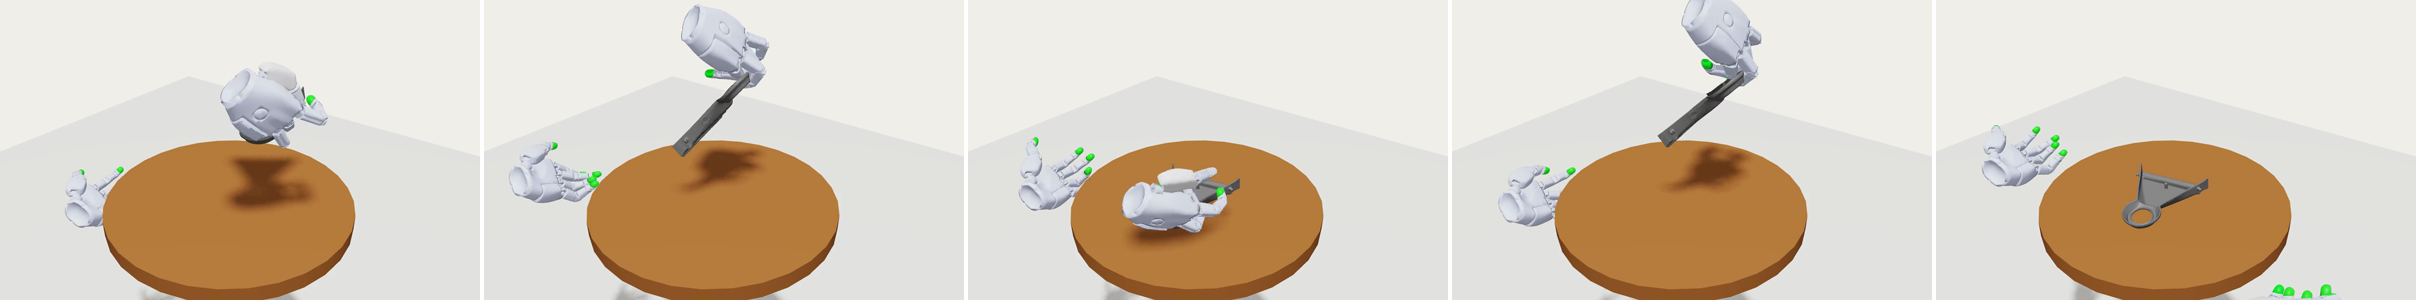
\includegraphics[width=0.9\linewidth]{figures/strip_e38.png}
  \caption{Learned policy re-enacting the dust-pan episode (eval ep.~38): grasp at the ring handle, carry, set down. This
  episode was never solved before simulator-settled starts and stickier contact (own-reference MP-SR 0\,$\rightarrow$\,0.98).}
  \label{fig:strip}
\end{figure*}

\section{Approach}
\label{sec:approach}

\paragraph{Perception.} We rectify the published colour-to-stereo extrinsic (3.4 vs.\ 18.9\,px reprojection error), run
FoundationStereo~\citep{wen2025foundationstereo} for metric depth and DROID-SLAM~\citep{teed2021droid} for ego-motion, and
fit the round table plane for gravity. A VLM, Qwen3-VL~\citep{bai2025qwen3vl}, describes the task from 8 frames and names each object with a short noun phrase (the
object identifier is a fallback); these phrases prompt SAM~3~\citep{carion2025sam3}, which segments objects and hands (masks
match the hand-written prompts within 0.02 IoU on 35/36 objects). Object meshes come from
SAM~3D Objects~\citep{chen2025sam3d} on automatically picked unoccluded views, metrically scaled by stereo depth; the
consensus of several samples is kept. Hands are Dyn-HaMR~\citep{yu2025dynhamr} MANO~\citep{romero2017mano} trajectories in metric scale;
the few frames it misses (3157392\%) fall back to WiLoR~\citep{potamias2025wilor} keypoints triangulated across the stereo pair.

\paragraph{Object trajectories (\method).} For every frame $t$ we keep all $K\!\approx\!252$ refined FoundationPose
hypotheses $X_t^k$ with scores $s_t^k$, instead of the argmax. TrackEverything~\citep{jain2026trackeverything} supplies
surface points $p_n(t)$ tracked in the SLAM world (seeded on object masks minus hand pixels). Following the multi-hypothesis
idea of Hand2Robot~\citep{du2026hand2robot}, we decode one hypothesis per frame by Viterbi,
\begin{equation}
\label{eq:viterbi}
\begin{aligned}
\min_{k_{1:T}} \sum_t \Big[&1 - \hat s_t^{k_t}\,\mathrm{IoU}_t^{k_t} + \lambda_p\, d_{\mathrm{surf}}(X_t^{k_t})\\
 &+ \lambda_m \textstyle\sum_n \big\| X_t^{k_t} (X_{t-1}^{k_{t-1}})^{-1} p_n(t\!-\!1) - p_n(t) \big\| \Big],
\end{aligned}
\end{equation}
where IoU ignores hand pixels (a covering hand is not evidence), $d_{\mathrm{surf}}$ is the distance of visible tracked
points to the hypothesis surface, and the pairwise term demands that consecutive hypotheses move the tracked points as they
actually moved; a flip or spin becomes expensive. Tracks are then anchored in the object frame so that points seen far apart
in time land on the same mesh location. Physical filters follow: a speed-limit Viterbi that keeps, flips or drops frames
($\leq$20$^\circ$, 6\,cm per frame), a rest hold for untouched objects, a spin guard letting held objects rotate only with
the holding hand plus slip (inspired by \citep{jeon2026vicon,shin2026compose}), and exact twist unwrapping for rotationally
symmetric cups. A VICON-style soft pose graph~\citep{jeon2026vicon} improved mocap accuracy slightly but cannot escape a
180$^\circ$ flip; we also considered~\citep{zhang2025tapip3d,tremblay2023diffdope,nguyen2025gotrack}.

\paragraph{Simulator grounding.} Reconstructed fingers sat 2--4\,cm inside cups, so reset shoved hand and cup apart; we
translate each hand (time-smoothed) out of every object. Resting objects carried a $\sim$12$^\circ$ tilt about the camera's
horizontal axis---the least observable direction---and tipped at reset; we drop each scene into the simulator for 2\,s
without the robot and adopt the settled poses as initial rests (accepted if $\leq$20$^\circ$/3\,cm). Collision is CoACD
\citep{wei2022coacd} on 4\,mm walls (openings stay open), a dish-rack slot is carved where the sweeper really stood, and
cups get a solid base. The pitcher mesh was lengthened at its base from a measurement (it rested 36\,mm above the table in
all three pitcher episodes).

\paragraph{Policy learning.} One FlashSAC~\citep{haarnoja2018sac,chordreport} policy per episode (2048 worlds,
250\,M steps, real-time playback) with the reward
$r = 40\,r_{\mathrm{obj}} + 5\,r_{\mathrm{cloc}} + 10\,r_{\mathrm{wrench}} + 5\,r_{\mathrm{prog}} + 200\,\mathbb{1}_{\mathrm{done}} - \ldots$,
i.e.\ object keypoint tracking, a contact-aware term rewarding robot fingers at the human contact locations and
contacts able to support the object, progress while every object is
within 3\,cm/0.3\,rad, and a completion bonus, with termination limits annealed from 3$\times$ to the official values. We
train two seeds and a stickier contact (friction 1.5) and submit, per episode, the run with the best own-reference
MP-SR, then SP-SR, then AUC.

\section{Experiments and Results}
\label{sec:experiments}

\begin{table}[t]
  \centering
  \small
  \setlength{\tabcolsep}{3pt}
  \resizebox{\linewidth}{!}{%
  \begin{tabular}{lcccccc}
    \toprule
    Submission & AUC$\uparrow$ & SP$\uparrow$ & MP$\uparrow$ & RPE$\downarrow$ & MPPE$\downarrow$ & CD-O$\downarrow$\\
    \midrule
    \method + pose filter & 0.504 & 0.50 & 0.15 & 9.23 & 8.60 & 0.407\\
    + physical filters, grounding & 0.532 & 0.55 & \textbf{0.20} & 8.10 & 7.82 & 0.407\\
    + 2nd seed               & 0.553 & 0.60 & 0.15 & 7.54 & 7.18 & 0.401\\
    + settled starts, friction & \textbf{0.584} & \textbf{0.65} & 0.15 & \textbf{7.35} & \textbf{6.06} & \textbf{0.401}\\
    \midrule
    leader                   & 0.765 & 0.80 & 0.50 & 3.85 & 3.00 & --\\
    \bottomrule
  \end{tabular}}
  \caption{Official test scores (20 evaluation episodes, own meshes). RPE, MPPE, CD-O in cm.}
  \label{tab:results}
\end{table}

Table~\ref{tab:results}
shows the official scores of successive submissions: every component improved AUC, SP-SR, RPE and MPPE
(about 12th of 37 by summed rank). SAC clearly outperformed PPO~\citep{schulman2017ppo} on identical data and reward
(median reference progress 0.62 after 250\,M steps vs.\ 0.27 after 492\,M; App.~\ref{sec:appendix}).
Simulator settling cut the mean rotation of resting objects during the first 3\,s from 12.3$^\circ$ to 5.0$^\circ$ and made
the dust-pan, sweeper and board episodes solvable (Fig.~\ref{fig:strip}). Two findings were negative: rigidly locking held
objects to the reconstructed palm lowered mocap accuracy (0.87$\rightarrow$0.55--0.72 of carried frames within 15$^\circ$/3\,cm),
because the palm frame drifts and objects genuinely slip; and hand-only refinement~\citep{liu2024geneoh} cannot repair object
poses. Most tellingly, 16 of 20 episodes pass MP-SR against our own reconstruction but only 3 against the hidden ground truth.

\balance

\section{Conclusion}
\label{sec:conclusion}

Global hypothesis selection with point-track consistency, plus simulator-side grounding, makes egocentric human motion
imitable by a dexterous robot hand; the remaining gap is reconstruction accuracy, especially the camera-depth tilt of resting
objects and centimetre offsets of held ones. Feeding simulator feedback back into the reconstruction (as in
DeepSimHO~\citep{wang2023deepsimho}) and refining meshes jointly with poses are the most promising next steps.
Code: \url{https://github.com/KiaRational/v2d-track3}.

\bibliographystyle{plainnat}
\bibliography{references}

\clearpage
\appendix
\section{Additional Results}
\label{sec:appendix}

\begin{figure*}[h]
  \centering
  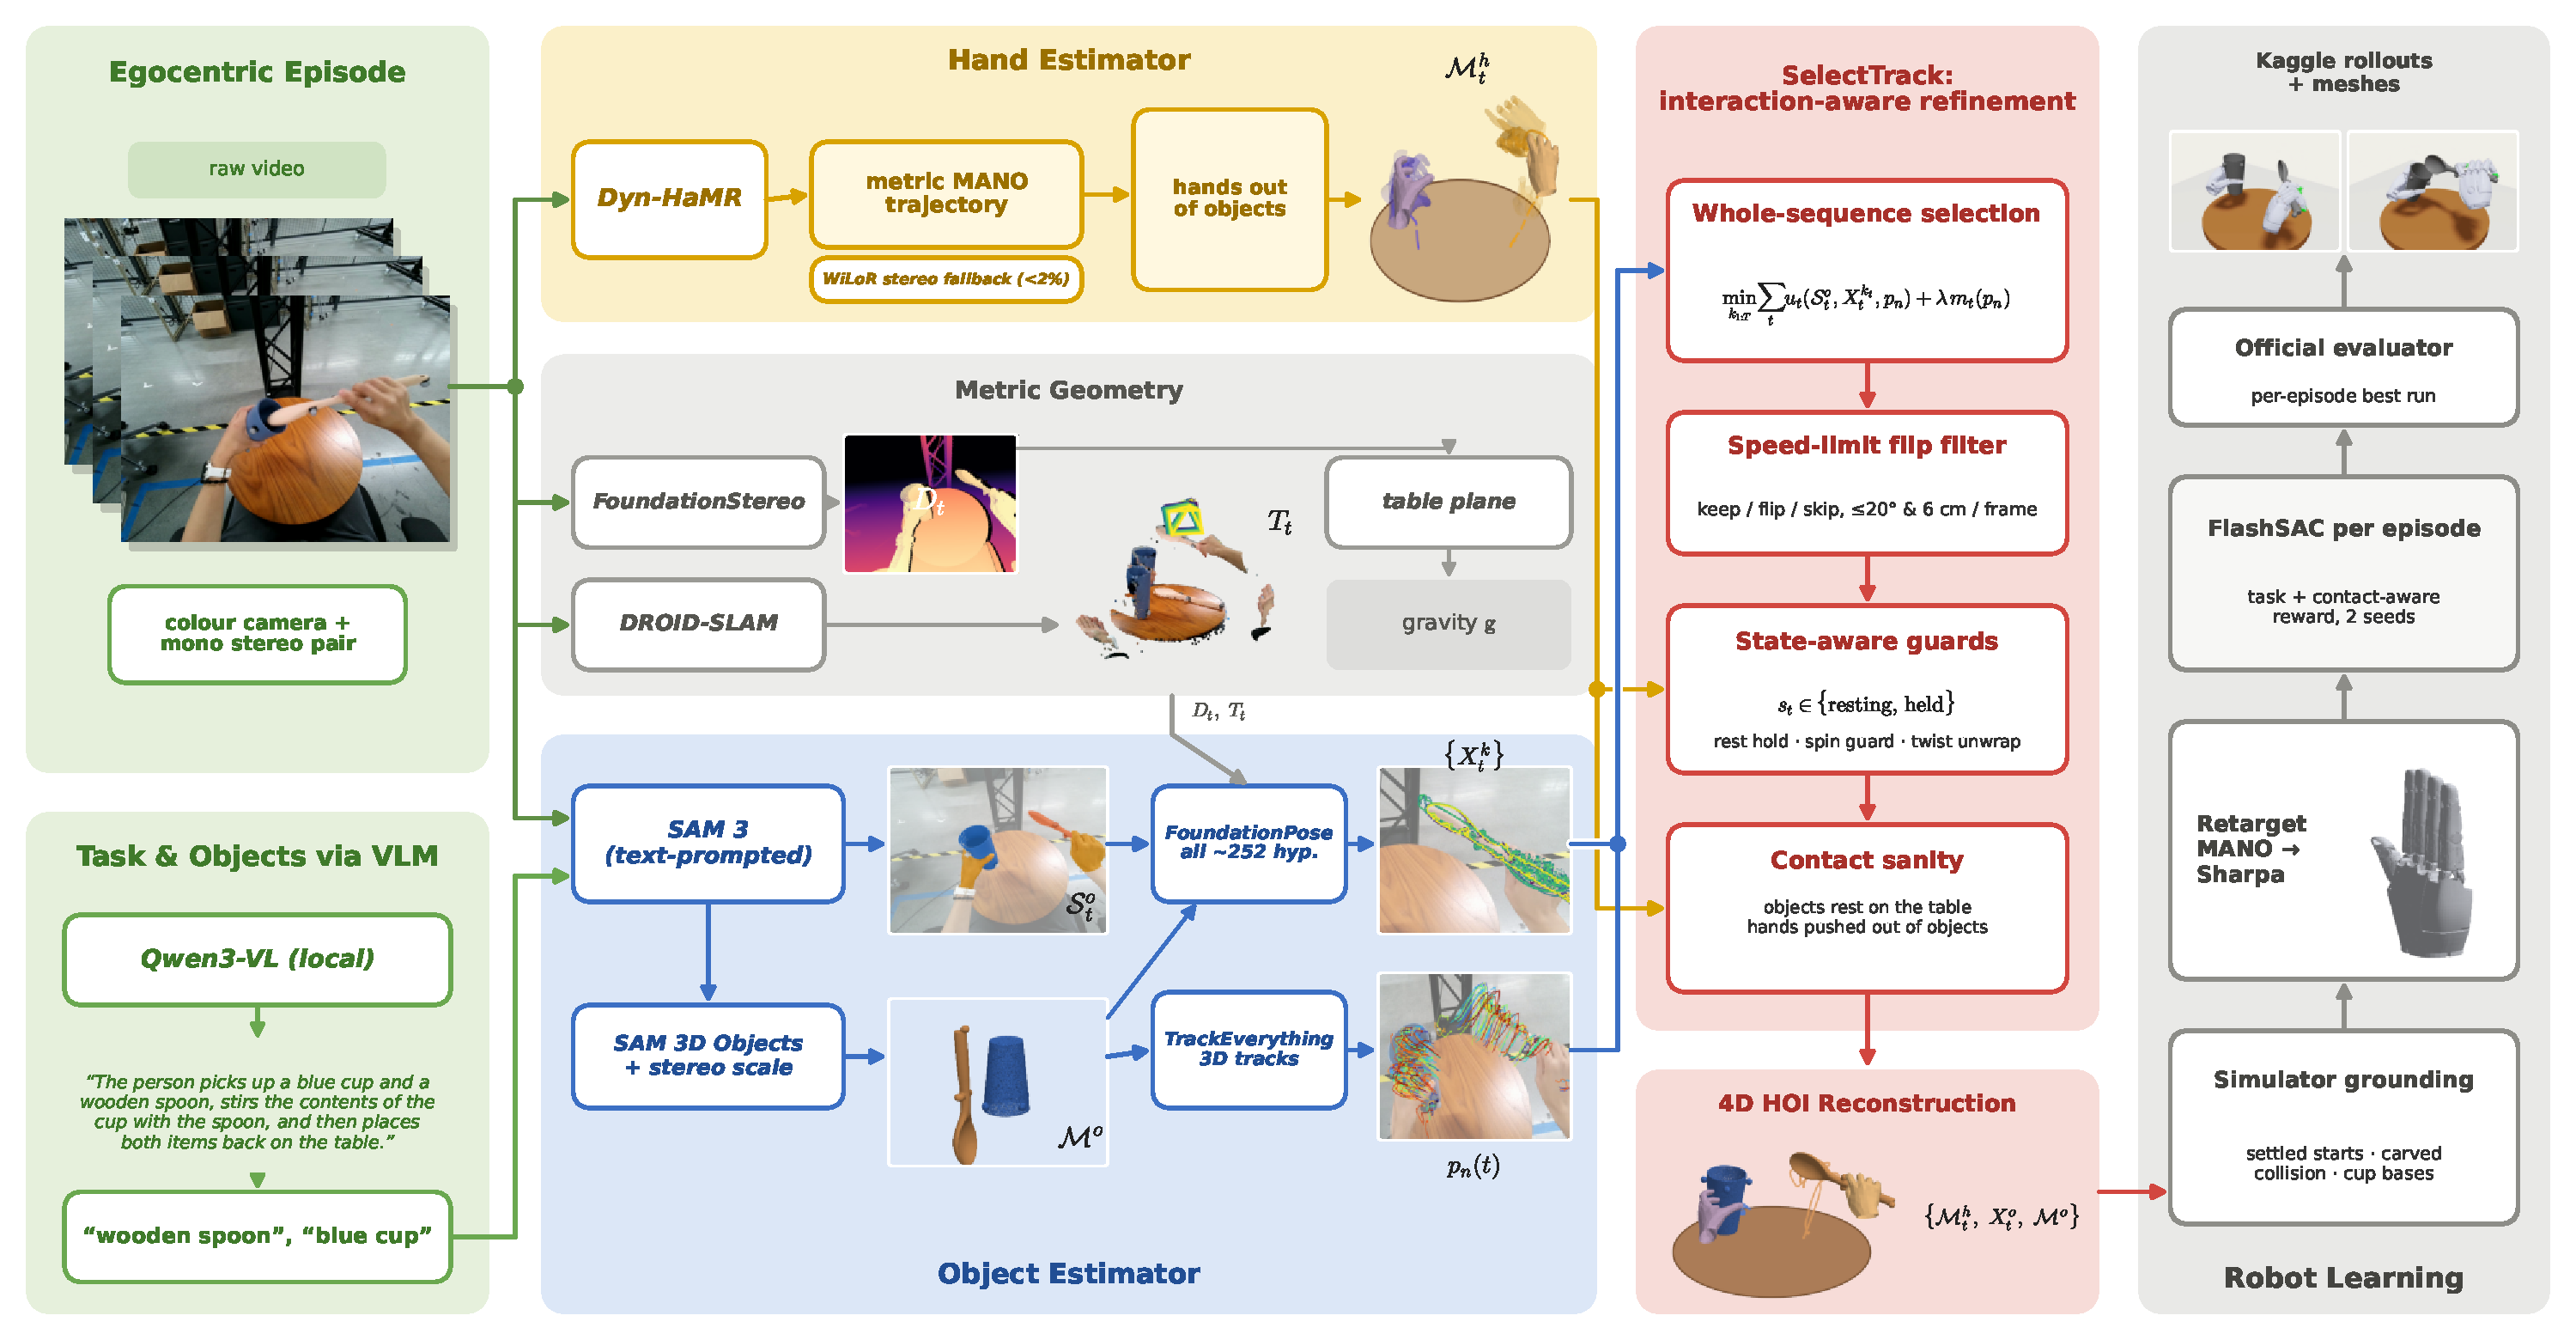
\includegraphics[width=\linewidth]{figures/arch.pdf}
  \caption{System architecture. A VLM names the objects for SAM~3; hand and object estimators produce MANO hands, meshes,
  all FoundationPose hypotheses and 3D point tracks; \method selects and grounds object trajectories; the 4D
  reconstruction is retargeted to Sharpa hands and a per-episode SAC policy is trained in simulation.}
  \label{fig:arch}
\end{figure*}

\begin{figure}[h]
  \centering
  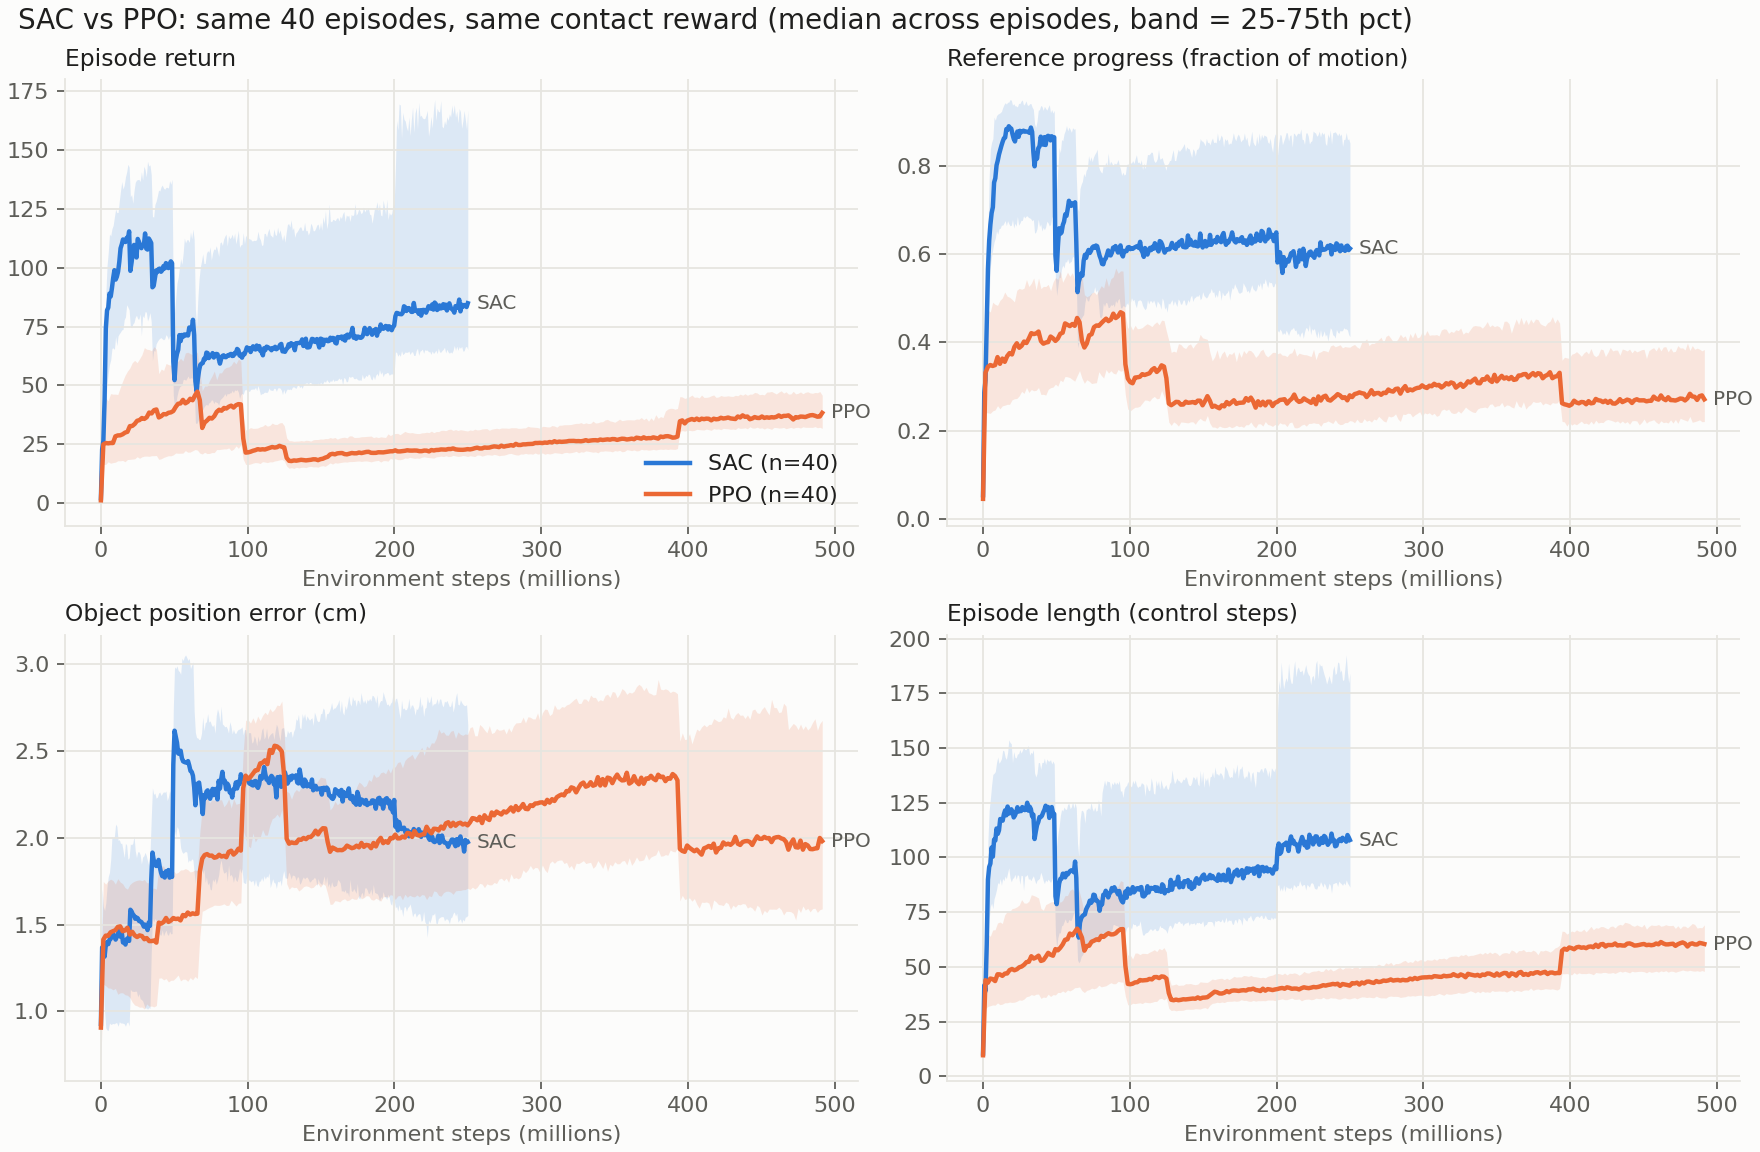
\includegraphics[width=\linewidth]{figures/fig1_sac_vs_ppo.png}
  \caption{SAC vs.\ PPO on the same 40 episodes and contact reward (median over episodes, band 25--75th percentile). Drops
  are curriculum stage changes (assistance reduced, termination tightened).}
\end{figure}

\begin{figure}[h]
  \centering
  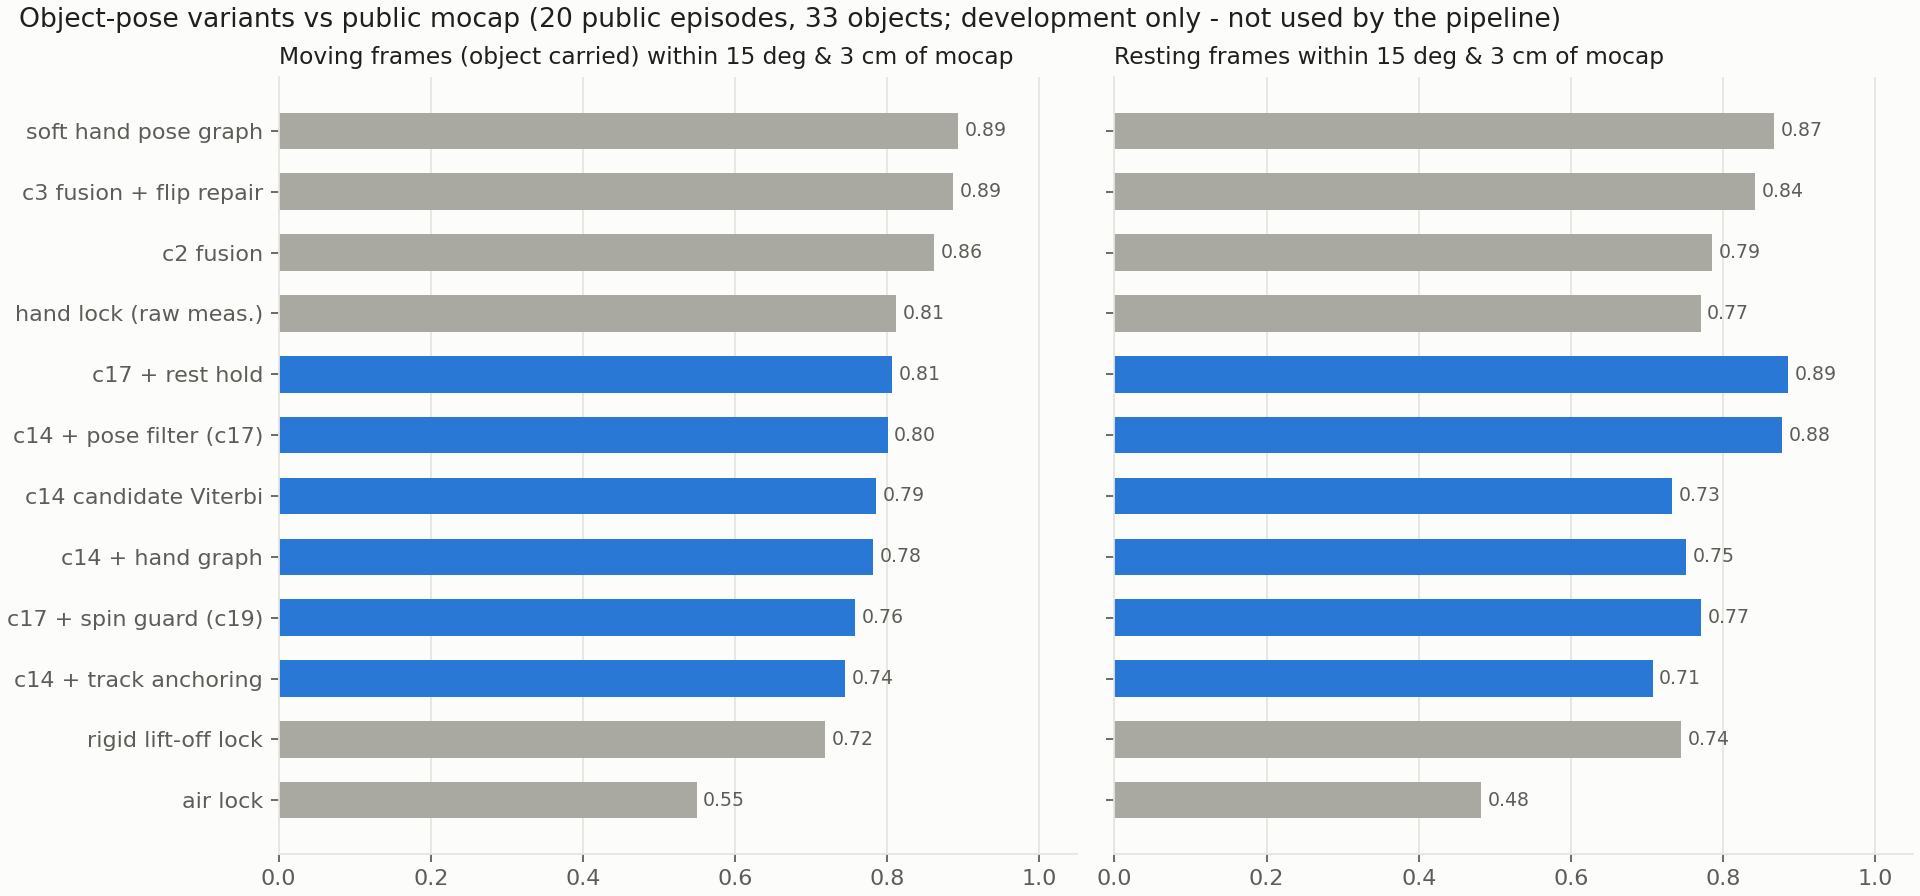
\includegraphics[width=\linewidth]{figures/fig9_pose_variants_mocap.png}
  \caption{Object-pose variants vs.\ public mocap (development only). \method trades a little carried-frame accuracy for
  the removal of flips and spins, which is what the robot needs.}
\end{figure}

\begin{figure}[h]
  \centering
  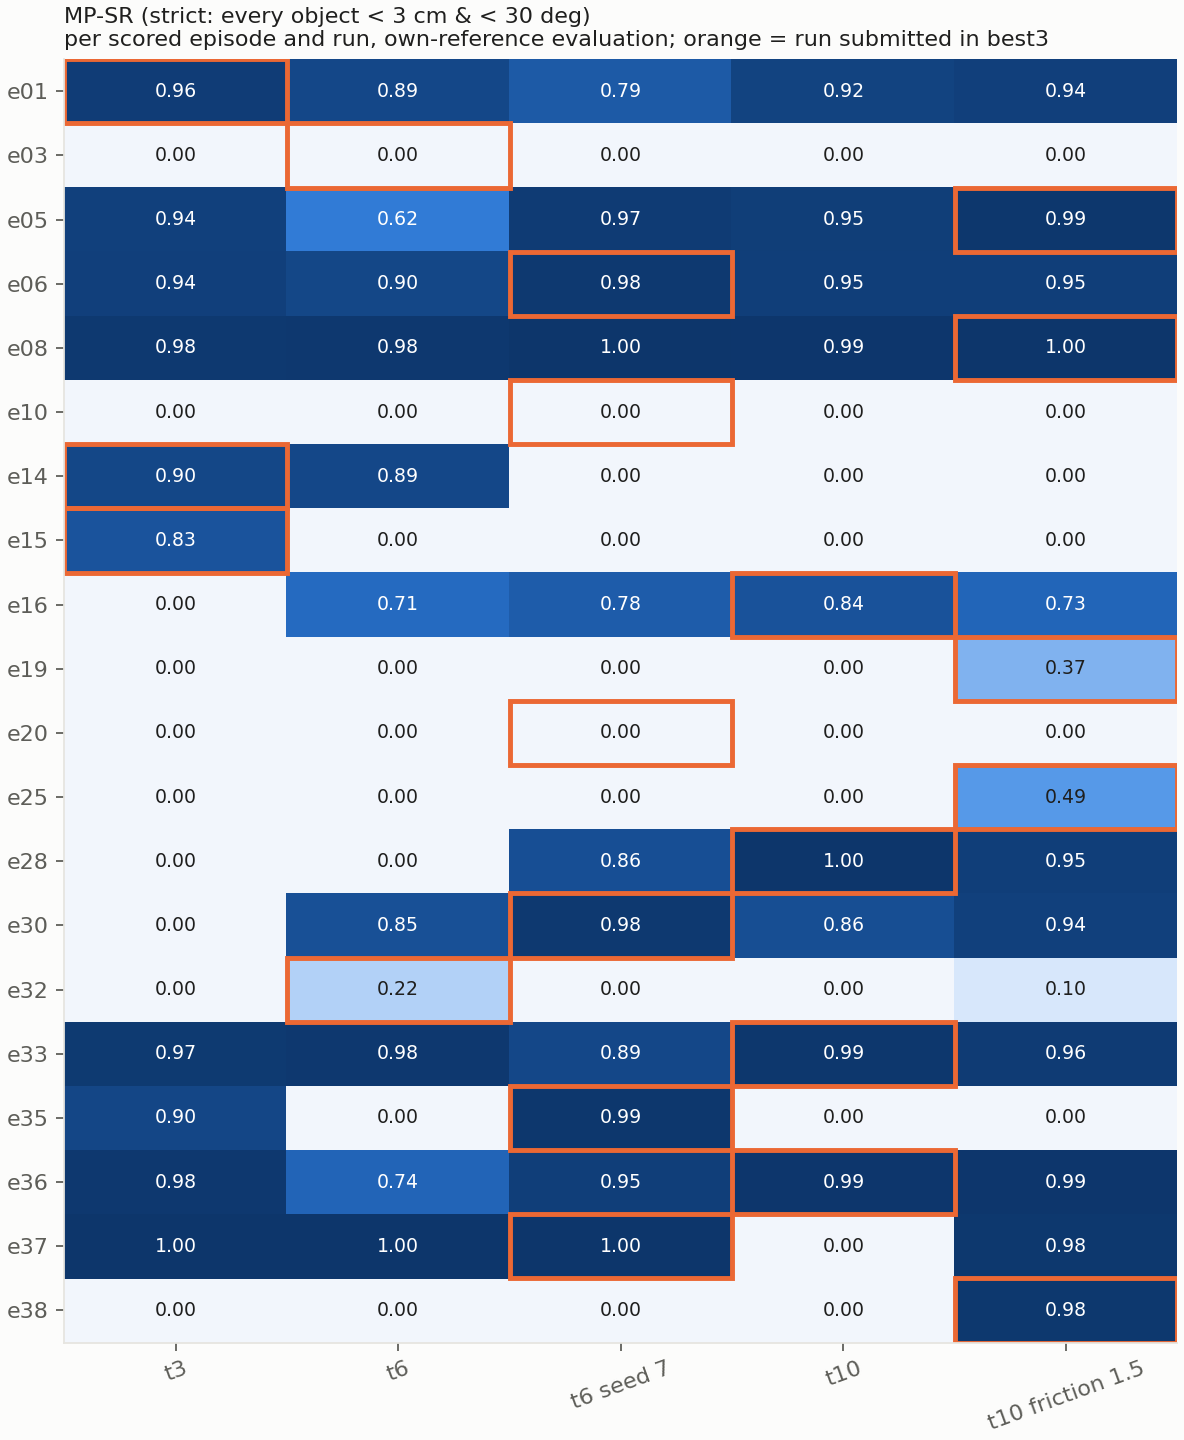
\includegraphics[width=0.8\linewidth]{figures/fig6_episode_mpsr.png}
  \caption{Own-reference MP-SR per scored episode and training run; outlined: run submitted.}
\end{figure}

\begin{figure}[h]
  \centering
  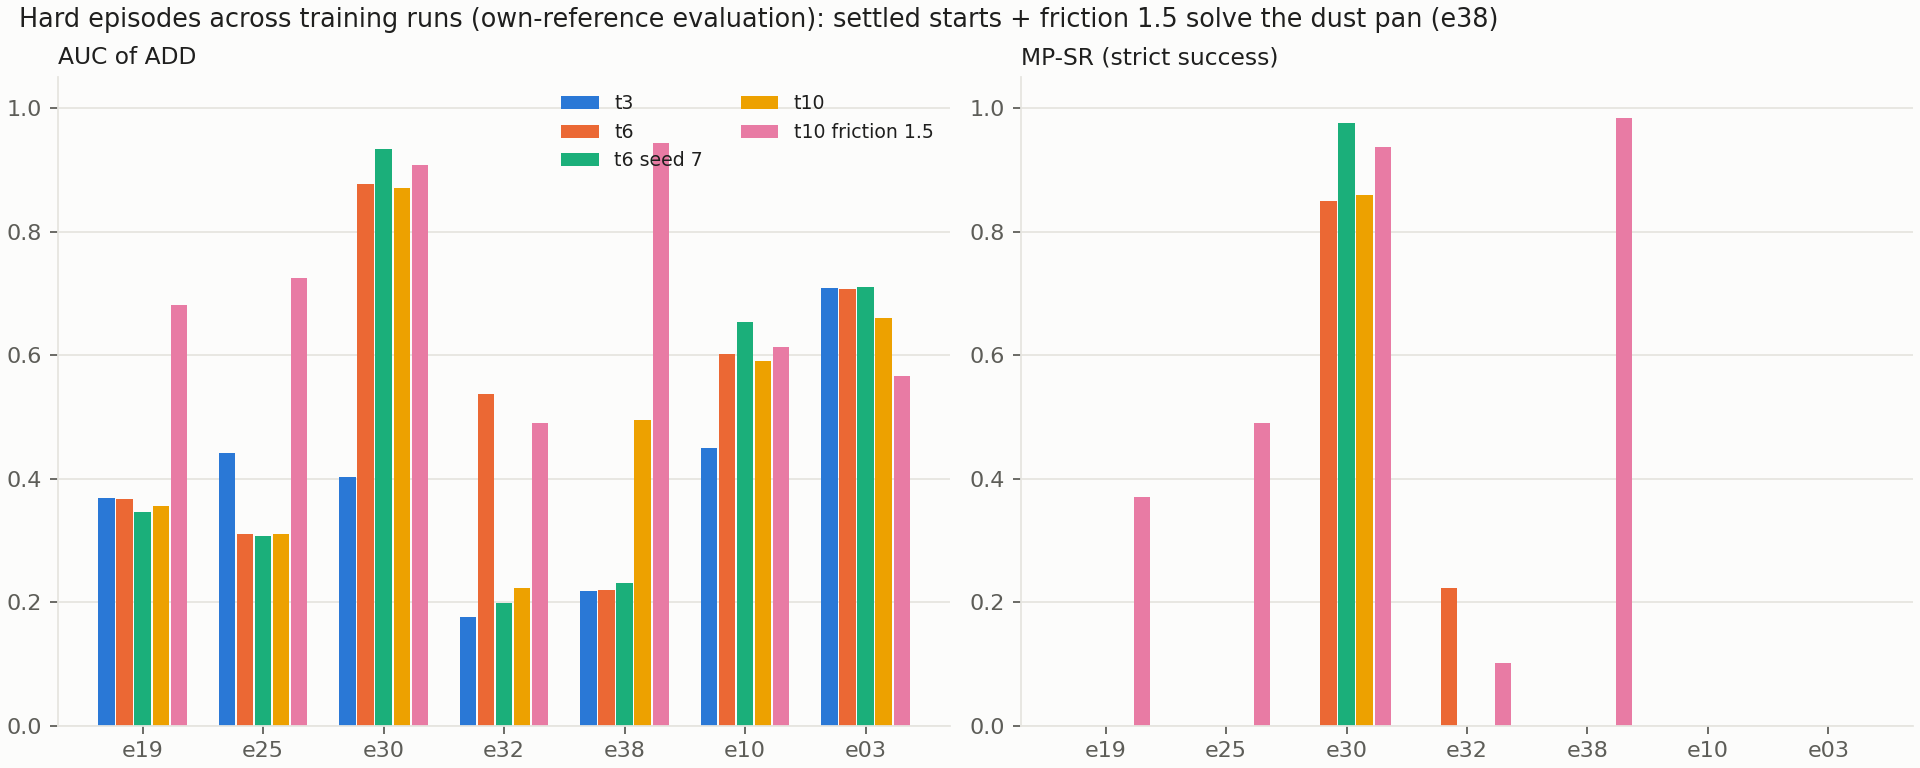
\includegraphics[width=\linewidth]{figures/fig11_hard_episodes.png}
  \caption{Hard episodes across runs: settled starts and friction 1.5 solve the dust pan (e38) and boards (e25).}
\end{figure}

\begin{figure}[h]
  \centering
  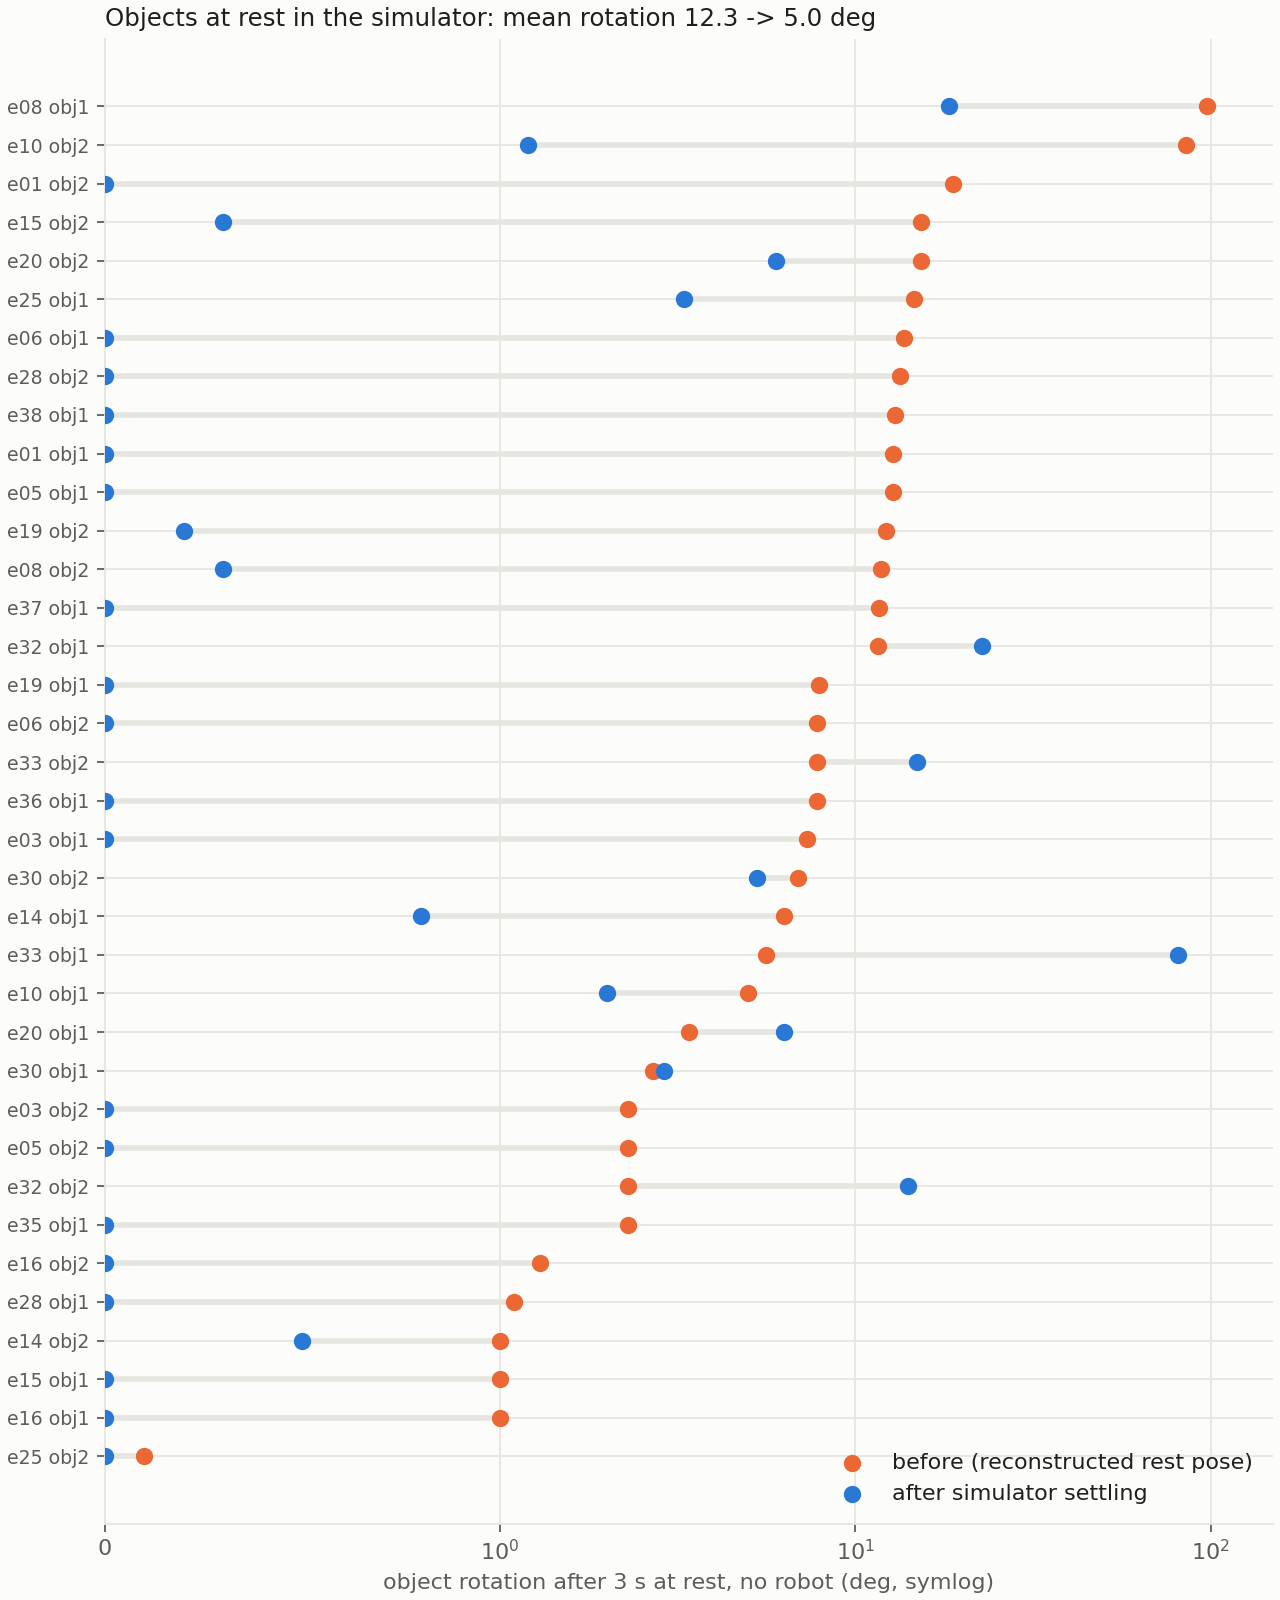
\includegraphics[width=0.75\linewidth]{figures/fig8_sim_settle.png}
  \caption{Rotation of each resting object over 3\,s without the robot, before and after simulator settling.}
\end{figure}

\end{document}
